\documentclass{article}
\usepackage{amsmath}
\usepackage{amssymb}
\usepackage{graphicx}
\usepackage{blindtext}
\usepackage{hyperref}
\usepackage{float}

\title{Analyse de solution : Station météo }
\date{2022\\ Décembre}
\author{Farah BALEHOUANE, Maxime GUY, Majdi RHIM\\ Master 1 Traitement de signal, Université de Poitiers}
\begin{document}
    \maketitle
    \section{Introduction}
    \blindtext
    \pagebreak
    \tableofcontents
    \part{Spécifications externes}
        \section{Mesure des précipitations}
            Les précipitations sont évaluées selon une période de temps : heure / jour / semaine / mois.
            Le capteur consiste en un réservoir couplé à un balancier \ref{fig:rain-sensor}. Un certain volume d'eau déclanche la vidange de ce dernier, son mouvement créer le contact sur un actionneur Reed à l'aide d'un aimant.\\
            \begin{figure}[H]
                \centering
                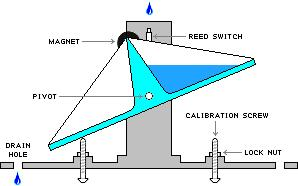
\includegraphics[scale=0.5]{img/rain_sensor/tipping-bucket-rain-gauge.jpg}
                \caption{Tipping bucket rain sensor}  \label{fig:rain-sensor}
            \end{figure}
            Le signal mesuré consiste en une série de pulsations à intervalles de temps irréguliers.
            Ce dernier est une entrée sur une PIN que l'on configurera en interruption externe avec détection de front montant/descendant.\\
            La donnée doit être traité de manière à garder la trace des interruptions dans le temps. Pour cela un tableau de date est maintenu:\\
            \begin{enumerate}
                \item A chaque intérruption une entrée est ajoutée sa valeur est la date de l'interruption en seconde depuis le 01:01:1970 00:00:00.
                \item Une variable par base de temps est incrémentee par la constante de hauteur de précipitation d'un réservoir durant l'itération du tableau si la valeur est inclue dans l'intervalle [instant de la mesure; instant de la mesure - période de la base].
                \item Si l'entrée du tableau est supérieur à la plus grande période, elle est fixé à 0 dans le but d'être supprimée.
            \end{enumerate}
            
            On obtiens alors une hauteur de précipitation par heure/jour/semaine/mois qui peut être utilisé pour l'affichage ou la sauvegarde des données.
        \section{Affichage des données}
    \part{Composition de l'application}	
        \section{Flot de données}
            \begin{figure}[H]
                \centering
                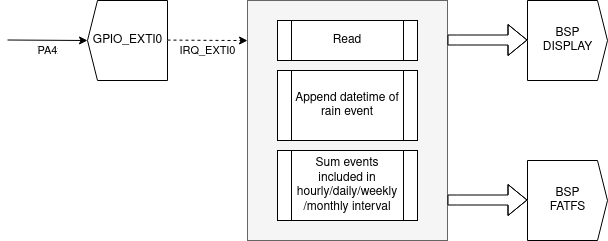
\includegraphics[width=0.8\columnwidth]{diagrammes/rain_fdd.drawio.png}
                \caption{Précipitations : Flôt de données}  \label{fig:fdd}
            \end{figure}
        \section{Flot d'évènements}
    \part{Développement}
        \section{Validation unitaire}
        \section{Validation des élléments d'assemblage}
            \subsection{Aggregation des mesures}
            \subsection{Gestion de l'IHM}
        \section{Validation de l'application}
    \part{Fonctionnalités réalisées}
    \part{Conclusion}
    \part{L'équipe projet}
    
\end{document}